\chapter{Methods}\label{chap:methods}

In this section, we dive into the specifics of the methodologies employed throughout the course of this thesis, providing a comprehensive overview of the technical aspects and methods undertaken. Each step of the methodology—from the data and preprocessing to evaluating the descriptions produced by the models—is thoroughly investigated to provide a clear and comprehensive explanation of the methods used in this research. Readers will obtain a deep understanding of the technical details and structure supporting the findings and analyses in later chapters by working through this section. 

To gain a thorough understanding of the entire pipeline (\autoref{fig:process_flow}), we will discuss the steps involved in generating a product description using an example. The product (\autoref{exmaple-product}) used in this illustration was chosen at random from among all products in the "Toner" category. The "Toner" category was chosen due to its ranking as one of the most abundant categories in our dataset. Furthermore, the creation of product descriptions for toners requires a certain level of knowledge and technical information, making them suitable for a detailed examination of our methods.

\begin{center}
	\fbox{\begin{varwidth}{\textwidth}
			\begin{flushleft}
				Product name: Lasertoner cyan OKI 42804547 \\
			Product category: Toner, Tonereinheit (Laserdrucker, Kopierer)
			\end{flushleft}
	\end{varwidth}}\par
	\captionof{Example}{The product used as a example \label{exmaple-product}}
\end{center}

\begin{figure}
	\centering
	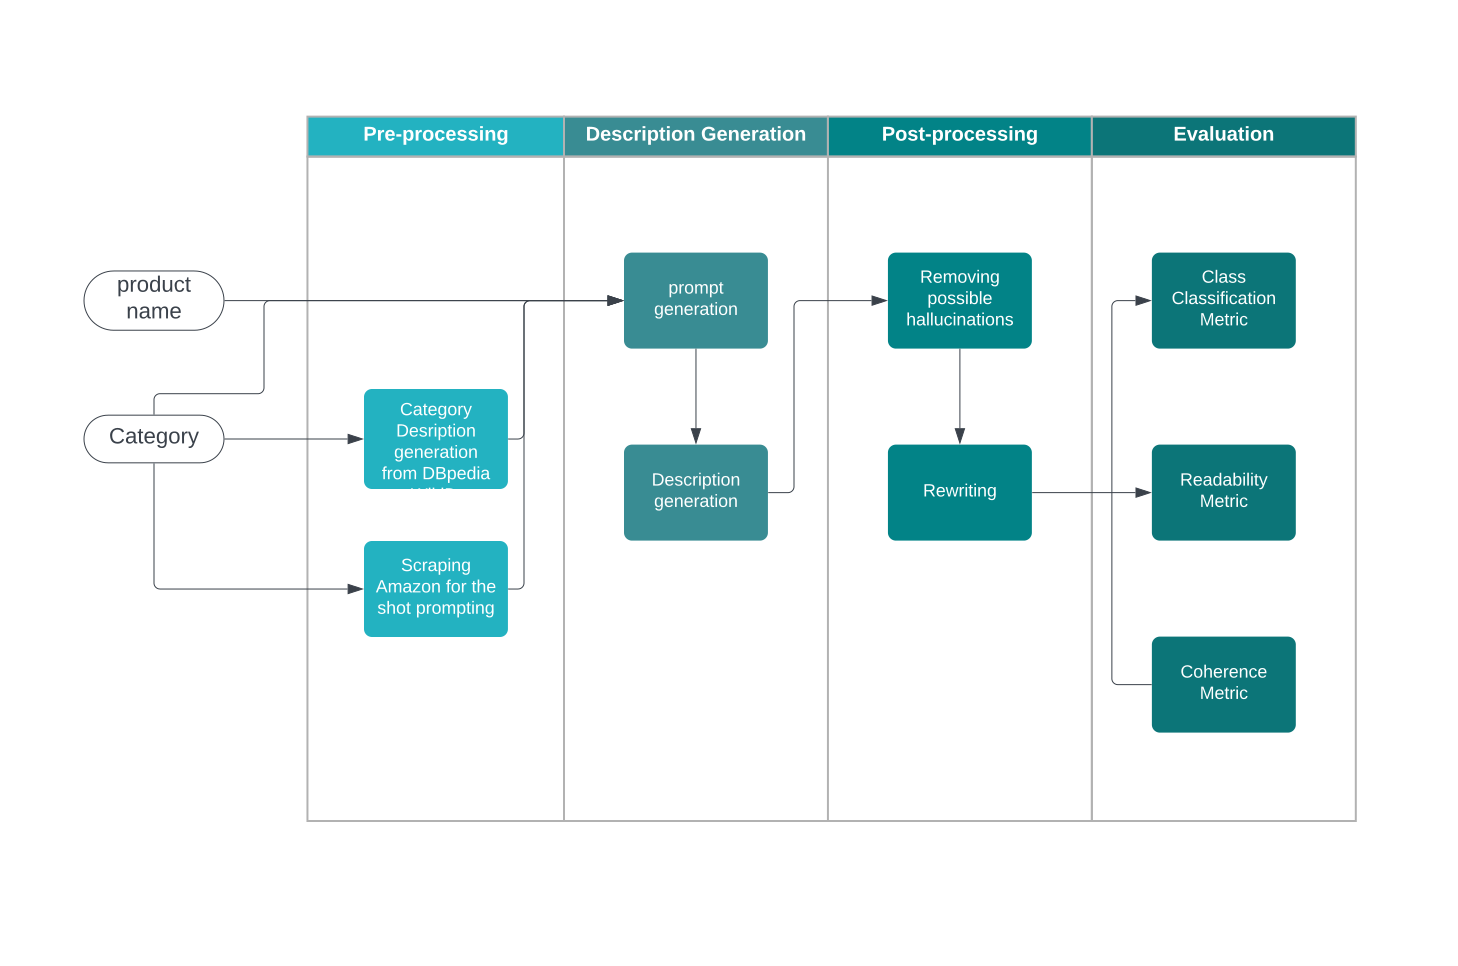
\includegraphics[width=1\linewidth]{process_flow}
	\caption{Process flow of the pipeline}
	\label{fig:process_flow}
\end{figure}

\newpage
% Describe the method/software/tool/algorithm you have developed here

\section{Dataset}

The dataset utilized in this research is taken from a collection provided by PBS, a leading distributor of paper, office, and stationery products in Central and Eastern Europe. 

PBS Holding AG is a prominent distributor in Europe, providing services to more than 200,000 clients in eight different European countries. PBS guarantees the smooth delivery of office supplies and paper products with a committed staff and regionalized logistics. With more than 1,400 workers, the company brought in an impressive €325 million in revenue in 2020.

With 231,630 entries, the dataset incorporates a combination of integer and object data types, with some fields having non-null values and others containing missing data. The hierarchical nature of the dataset is evident, reflecting the diverse range of products distributed by PBS. The table (\autoref{tb:dataset}) shows a small subset of the dataset. The columns are as follows:


\begin{enumerate}
	\item Konzernartikelnummer: Unique identifier for each product within the catalog.
	\item ECLASS\_8\_1: ECLASS classification code associated with the category of the product.
	\item ECLASS\_Name: Descriptive name corresponding to the ECLASS classification.
	\item Bezeichnung: Product names.
	\item Webbezeichnung: Name used for online presentation of the product.
	\item Detailinformation: Detailed information about the product. equivalent to the product description
	\item LieferantenDetailinformation: Supplier-specific details about the product.
	\item OEMNummer: Original Equipment Manufacturer (OEM) number linked to the product.
	\item Hersteller: Manufacturer of the product.
	\item Marke: Brand associated with the product.
\end{enumerate}


	
	
\begin{landscape}
	\begin{table}[!ht]
		\centering
		\tiny
		\begin{tabularx}{\linewidth}{
				|>{\centering\arraybackslash}X
				|>{\centering\arraybackslash}X
				|>{\centering\arraybackslash}X
				|>{\centering\arraybackslash}X
				|>{\centering\arraybackslash}X
				|>{\centering\arraybackslash}X
				|>{\centering\arraybackslash}X
				|>{\centering\arraybackslash}X
				|>{\centering\arraybackslash}X
				|>{\centering\arraybackslash}X|} 
			\hline
			\textbf{Konzernartikel-nummer} & \textbf{ECLASS\_8\_1} & \textbf{ECLASS\_Name} & \textbf{Bezeichnung} & \textbf{Web-bezeichnung} & \textbf{Detail-information ( the one online)} & \textbf{Lieferanten-Detail-information (the company)} & \textbf{OEMNummer} & \textbf{Hersteller} & \textbf{Marke} \\ \hline
			2766168000 & 24292401 & Standardkarteikarte & Karteikarte zu 20Bl. A4 SIGEL LP701 & Karteikarte zu 20 Stück A4 SIGEL LP701 & 160 Karten A7 blanko weiß,zum Selbergestalten am PC & PC- Karten weiß zum beidseitigen Bedrucken mit InkJet- und Laser-Drucker sowie zum Kopieren geeignet. Aufgrund der feinen Mikroperforation lassen sich die Karten schnell und einfach aus dem A4-Bogen lösen. Im Lieferumfang sind 20 Blatt à 8 Stück im Format DIN A7 enthalten. & LP701 & SIGEL GMBH & SIGEL \\ 
			1000255650 & 24360202 & Konferenzmappe & Schreibmappe A4 blau LEITZ 4580-00-37 Bebop & Schreibmappe A4 blau   Bebop LEITZ 4580-00-37 & m. Schreibblock u. Ablagefächern, 4 Sichthüllen, Stiftelasche,CD-u.Visitenkarten-tasche, m. Schreibblock, 40BL lin., perforiert,1 Fach f. Utensilien. 4 Sichthüllen mit Beschriftungstaben. Inkl. Beschriftungsschildchen. High-Tech Material-Mix: langlebiges PP in Opaque mit schimmerndem Perlmutt-Effekt. Neuartige Oberflächen-struktur: mit 3D-Prägeart. Innenseite: Grau-Ton. & Leitz Schreibmappe Bebop, mit liniertem Schreibblock, perforiert, 40 Blatt, mit Utensilienfach und Stiftelasche, 4 Sichthüllen mit Beschriftungsschildchen, mit CD-Tasche an der Klappe des Vorderdeckels. Oberflächen-struktur in 3D-Prägeart, mit Duo-Optik: leuchtende Außenfarbe, Innenseite in warmem Grau-Ton. Material: Polyproplyen (PP) mit Perlmutt-Effekt. Format: 320 x 240 x 26 mm. Farbe: blau. & 4580-00-37 & Esselte Office Products GmbH & LEITZ \\ 
			1000228410 & 19140605 & Tintenkartusche, Druckkopf (Tintenstrahldrucker) & Inkjetpatrone T5961 foto sw EPSON C13T596100 350ml & Inkjetpatrone T5961 foto schwarz   350ml EPSON C13T596100 & Inhalt: 350 ml, Epson Ink Stylus Pro 7900/9900, photo black, 350ml, T5961 & ~ & C13T596100 & UFP Austria GmbH & EPSON \\ \hline
		\end{tabularx}
		
		\caption{PBS product dataset in German language \label{tb:dataset}}
	\end{table}
\end{landscape}		

In the dataset, "Bezeichnung" refers to the product label, whereas "Webbezeichnung" is a manually edited version tailored for online presentation, ensuring an optimized and appealing representation for web visibility. The dataset features "Detailinformation" and "LieferantenDetailinformation," with the former often being a version, whether identical, rewritten, or adapted, of the latter.


PBS employs a hierarchical classification structure, with an 8-digit number indicating the product's category and subcategories. For instance, the first two digits represent the primary class, and subsequent pairs describe specific layers within that class. The top-level categories, including Büromaterial, Papier, Büroküche \& Hygiene, Tinte \& Toner, Möbel \& Einrichtung, Bürotechnik, and Geschenke, offer a comprehensive classification system for the products.

The dataset encompasses various product eclasses, with the top most repeated categories including Glückwunschkarte, Trauerkarte, Toner, Papier-Motivserviette, Geschenkband, and Geschenkartikel as visible in the figure (\autoref{fig:top_eclasses}).

\begin{figure}[H]
	\centering
	\includegraphics[width=1\linewidth]{top\_eclasses}
	\caption{The top 10 most repeated ECLASSES in the PBS Dataset}
	\label{fig:top_eclasses}
\end{figure}

In the upcoming sections, we will explain the techniques utilized in making use of this dataset to effectively address our research questions.


\section{Pre-processing}

In preparation for the subsequent stages of our research, an effective preprocessing pipeline is vital to refine and structure the raw data. The preprocessing phase primarily revolves around enhancing the dataset's informational depth by incorporating category descriptions and crafting few-shot prompting examples for the model. Firstly, Using PBS's hierarchical classification, we dynamically generate detailed category descriptions from Wikidata and DBpedia. This step improves the dataset, providing the model with contextual information for improved text generation. For the next step, real-world product descriptions are scraped from Amazon, creating diverse examples for each category. In the following subsections, we will dive into the processes and reasons for each of these steps.

\subsection{Category Description}

Generating informative category descriptions is pivotal for enhancing the contextual understanding of product categories within the dataset. Leveraging PBS's hierarchical classification system, each product's category is mapped to its corresponding Wikidata \cite{wikidata} and DBpedia \cite{dbpedia} entries. This dynamic process provides a detailed and structured description, encompassing the category's features, applications, and distinctive attributes.

The generated descriptions offer a contextual backdrop, providing detailed insights into the nature and purpose of each product category. This contextual enrichment aids the model in comprehending the inherent characteristics of diverse categories.

Additionally, During the text generation process, the model can draw upon the category descriptions to create more contextually relevant and linguistically coherent product descriptions. This contributes to the overall quality and informativeness of the generated text, aligning with the goal of creating engaging and accurate product descriptions.

The idea comes from the paper \cite{Chen_2019} (\autoref{Automatic_Product_Description_Generation}) where they introduce KOBE. The main components of the KOBE model are Attribute Fusion and Knowledge Incorporation. Attribute Fusion integrates product aspects and user categories with the title representation, while Knowledge Incorporation incorporates relevant knowledge retrieved from a knowledge base. The process of knowledge incorporation in product description generation involves seamlessly blending basic product information with relevant external knowledge, mirroring how humans draw upon their commonsense knowledge when describing products. To enhance product descriptions, They integrate external knowledge with basic product information by firstly sourcing Relevant knowledge from CN-DBpedia by matching product title words to named entities, creating a concatenated knowledge sequence. Then a Knowledge Encoder processes retrieved knowledge, producing a high-level representation. Employing bidirectional attention flow, this representation is fused with the product title, enriching descriptions by incorporating external knowledge. 


To generate category descriptions, we initially match the English category name with Wikidata entities, translating the description upon a successful match. Alternatively, we search DBpedia, examining result descriptions and applying rules, such as having the word "is" after the entity name; if this rule is met, we translate and use it as the category description. When a category name is extremely specific, such as "Kugelschreiber mit Befestigung," we search higher up the ECLASS hierarchy for an acceptable description. The following (\autoref{exmaple-category-description}) is the category description generated for the sample product (\autoref{exmaple-product})

\begin{center}
	\fbox{\begin{varwidth}{\textwidth}
			
			Pulver, das in Laserdruckern und Fotokopierern verwendet wird, um den gedruckten Text und die Bilder zu formen
	\end{varwidth}}\par
	\captionof{Example}{\label{exmaple-category-description} The category description generated for the sample product (\autoref{exmaple-product}) }
\end{center}

\subsubsection{Translation}

A critical step in the process of generating category descriptions is translating English descriptions into German to ensure linguistic consistency. To accomplish this, we used Python's "translators" library, which provides a variety of translation engines. Following careful evaluation, our findings indicated that the Bing translation engine outperformed the alternatives. As a result, we use Bing Translator for all of our translations.

\subsection{Shots}

Few-shot prompting is a pivotal aspect of our methodology, which involves providing a language model with a limited number of examples or instances to guide its generation, allowing it to adapt and generate relevant content based on the provided context. We employ a scraping mechanism to gather two illustrative product descriptions from the Amazon website within the same category as the input product. This approach aids the model in generalizing from a handful of instances to effectively describe a wide range of products within a specific category. The utilization of few-shot prompting contributes to the adaptability and versatility of our language model, enabling it to produce coherent and contextually relevant product descriptions even if it was not trained for this task.

Using related category examples in few-shot prompting is a more effective strategy than including unrelated instances. Our research, which will be discussed further in the Discussion section, demonstrates the significant impact of using examples from closely related categories. Preliminary results show that prompts with related examples are better able to generate accurate and contextually relevant product descriptions within the target category. Using unrelated examples, on the other hand, frequently results in descriptions that are unsuitable for the specified category, resulting in content misalignment and poor model performance. This highlights the significance of carefully chosen and category-specific examples in improving the model's ability to generate relevant and precise descriptions for a given product category.

Our approach to prompt engineering includes three variations: zero, one, and two-shot prompting, each of which provides the model with different levels of contextual information. Descriptions based on a single example may exhibit a desirable balance, showcasing a higher level of creativity tailored to the specific product. However, the effectiveness of these shots depends on the quality and clarity of the provided examples. If the shots lack precision or clarity, they may lead to confusion within the model, making the zero-shot approach preferable for ensuring consistency and accuracy in product descriptions.

\begin{center}
	\fbox{\begin{varwidth}{\textwidth}
			
			Produktname: Xerox Laser Toner Everyday 006R03838 Black Ersatz für HP CE505A diverse Canon ImageCLASS imageRUNNER LPB3470 LPB3480 LASER CLASS 650i P2035 P2055, \\
			
			Produktkategorie: Toner, Tonereinheit (Laserdrucker, Kopierer),\\
			
			Katagoriebeschreibung: Pulver, das in Laserdruckern und Fotokopierern verwendet wird, um den gedruckten Text und die Bilder zu formen,\\
			
			Produktbeschreibung :  Kapazität in Seitenzahl bis zu 2300 Seiten möglich Kompatibel mit Drucker Modell HP CE505A diverse Canon ImageCLASS imageRUNNER LPB3470 LPB3480 LASER CLASS 650i P2035 P2055 Wert: deutlich niedrigere Preise und deutlich niedrigere Kosten pro Seite als Originale Drucker Patrone Zuverlässig: ohne Fehler scharfe Bildqualität und außergewöhnliche Zuverlässigkeit einer Marke die Sie kennen und vertrauen Risikofrei: Xerox Everyday Tonerkartusche hat gegenüber den originalen Lasertoner keine Nachteile 
	\end{varwidth}}\par
	\captionof{Example}{\label{exmaple-shot} An example shot generated for the sample product (\autoref{exmaple-product})}
\end{center}




\section{Description Generation}

This section explores the complexities of our description generation process, explaining the careful design of prompts, parameters used for generation, and the model that is used. The creation of an effective prompt is critical, as it influences the model's understanding and subsequent output. We go into the factors that influenced our prompt design, highlighting the specific parameters that were chosen for maximum performance. Furthermore, we provide an overview of the architecture and capabilities of the chosen model, explaining the elements that motivate our approach.

\subsection{Prompt}


Our prompting technique involves a structured approach incorporating product names, categories, category descriptions, and examples to guide LLMs in generating product descriptions. Through experimentation, we found that including these elements in the prompt yields more stable and improved results, as indicated by human evaluations. The integration of product features, categories, and relevant examples enhances the LLM's understanding of the task, resulting in more contextually relevant and informative product descriptions.

The following is an example of the prompt generated for the sample product (\autoref{exmaple-product}). Based on the study that we did on the different subsets of features available in the PBS dataset and using them in the prompt, it was apparent that the usage of the other features such as "Marke" can lead to confusion of the model and therefore decided to not include them in our prompt. Additionally in another study, different sentences were used to explain the task to the model; However based on human evaluation, we could see that the straightforward and clear prompts leads to a more appropriate product description. This might be due to the fact that the model we're using isn't particularly complex—it only has 6 billion parameters. 

{\tiny
\begin{lstlisting}[breaklines=true, caption={a sample prompt}, captionpos=b]
	
	Schreib die Produktbeschreibung für das folgende Produkt. Hier sind zwei Beispiele:
	
	Produktname: DogePro TL-410 Tonerkartusche Schwarz Ersatz für PANTUM Laserdrucker P3300/P3308/P3018/M6800/M6808/M7100/M7100/M7108/M7200 (Schwarz, 1 -Pack),
	
	Produktkategorie: Toner, Tonereinheit (Laserdrucker, Kopierer),
	
	Katagoriebeschreibung: Pulver, das in Laserdruckern und Fotokopierern verwendet wird, um den gedruckten Text und die Bilder zu formen,
	
	Produktbeschreibung :  Kompatible Produkte: Pantum P3300DW, P3308DW, P3300DN, P3308DN, P3018DW, P3018DW, P3020D, M6800FDW, M6808FDW, M7100DW, M7108DW, M710DN. M710, M710, 8DN, M7200FDW, M7208FDW Geschätzte Seitenleistung: 1500 Seiten pro Patrone bei 5% Deckung (Brief, A4) Lieferumfang: 1 Packung TL-410 Tonereinheit Befolgen Sie die Installationsanweisungen, stellen Sie sicher, dass Sie die Schutzfolien entfernen und richtig installieren, ohne die mechanischen Teile des Druckers zu belasten. Bei Bedarf zögern Sie nicht, unseren technischen Support zu kontaktieren!
	
	
	Produktname: Xerox Laser Toner Everyday 006R03838 Black Ersatz für HP CE505A diverse Canon ImageCLASS imageRUNNER LPB3470 LPB3480 LASER CLASS 650i P2035 P2055,
	
	Produktkategorie: Toner, Tonereinheit (Laserdrucker, Kopierer),
	
	Katagoriebeschreibung: Pulver, das in Laserdruckern und Fotokopierern verwendet wird, um den gedruckten Text und die Bilder zu formen,
	
	Produktbeschreibung :  Kapazität in Seitenzahl bis zu 2300 Seiten möglich Kompatibel mit Drucker Modell HP CE505A diverse Canon ImageCLASS imageRUNNER LPB3470 LPB3480 LASER CLASS 650i P2035 P2055 Wert: deutlich niedrigere Preise und deutlich niedrigere Kosten pro Seite als Originale Drucker Patrone Zuverlässig: ohne Fehler scharfe Bildqualität und außergewöhnliche Zuverlässigkeit einer Marke die Sie kennen und vertrauen Risikofrei: Xerox Everyday Tonerkartusche hat gegenüber den originalen Lasertoner keine Nachteile 
	
	
	Schreib nun die Produktbeschreibung für dieses Produkt.
	Produktname: Lasertoner cyan OKI 42804547,
	Produktkategorie: Toner, Tonereinheit (Laserdrucker, Kopierer),
	Katagoriebeschreibung: Pulver, das in Laserdruckern und Fotokopierern verwendet wird, um den gedruckten Text und die Bilder zu formen,
	Produktbeschreibung:
	
\end{lstlisting}
}


While exploring additional parameters, we introduced a prompt style variable, including formal, simple, scientific, and other styles. However, our experiments revealed that manipulating prompt style had a negative impact on the overall results. As a result, in our final experiments, we decided to exclude the prompt style parameter to ensure a more straightforward and effective approach to product description generation.


\subsection{Text Generation}


Text generation involves the application of LLMs, particularly in our case by leveraging the Transformers Python library. Transformers (\autoref{Transformers}) are a type of neural network architecture that excels at processing sequential data, making them highly suitable for NLP tasks. In our text generation process, we employ the Transformers library's pipelines, which provide a simple and efficient interface for utilizing pre-trained models.

In our specific pipeline, we utilize the BLOOM-CLP German model (\autoref{german-bloom}), which has 6.4 billion parameters, enabling it to capture intricate language patterns and generate coherent and contextually relevant text in German. The parameters employed in our pipeline include a temperature setting of 0.8, controlling the randomness of the generated text, while the max\_new\_tokens parameter is set to 150, limiting the length of the generated output. We conducted a study to see the influence of different temperatures on the output and based on that study we decided to go with 0.8 since it had shown the most robustness for different products. Additionally, Larger max\_new\_tokens will lead to hallucination and false information in the output. The do\_sample parameter is enabled, meaning that we would use the sampling as our decoding strategy. In sampling, model randomly selects the next token based on the probability distribution over the entire vocabulary provided by the model, as opposed to greedy search, which the model always selects a token with the highest probability as the next token. Additionally, a repetition\_penalty of 4.0 is employed to discourage the model from producing repetitive sequences, contributing to more diverse and engaging generated text. Based on our extensive experiments, this combination of parameters ensures an effective and controlled text generation process tailored to our specific requirements. The description (\autoref{exmaple-description}) was generated using the parameters we discussed above for the sample product (\autoref{exmaple-product}).

\begin{center}
	\fbox{\begin{varwidth}{\textwidth}
			 \begin{flushleft}
			 	Die Tintenpatron ersetzt Original TN2260C aus dem Hersteller Okiexperts Orignal OEM Nummer O42 80 45 47. Diese neue tintenkartuschen bieten Ihnen höchste Qualität zum günstigen Preis sowie absolute Funktionssicherheit von Markenherstellern wie Ricoh oder Kyocera im Vergleich zur preiswerten Kopie! Dieser original kompatiblert Farbtonersatz besteht komplett ausschließlich nur besten Komponenten, welche garantieren daß man eine Spitzenqualität beim drucken bekommt!! Für Ihren Lieblingstank erhalten sie ein Garantiert Zufriedenheits Garantie auf alle unsere angebotenen Patronen vom ersten Einkauf an.. Im Rahmen dieser Rückgabegarantie können Kunden innerhalb eines Monats nach Erhalt ihrer Bestellung gegen Vorlage ihres Kassenzettel zurückgeben falls es Probleme geben sollte egal ob Ihr Ausdruck durch falsche Verwendung Ihrer neu eingekauf
			 \end{flushleft}
	\end{varwidth}}\par
	\captionof{Example}{The description generated for the sample product \label{exmaple-description} (\autoref{exmaple-product})}
\end{center}

\section{Post-processing}

Post-processing plays a crucial role in refining the output of our text generation model to ensure the generated descriptions meet the desired criteria. In this phase, our focus is on addressing potential issues such as hallucinations—instances where the model generates information that is not contextually relevant or accurate. We implement measures to carefully filter and curate the generated text, removing any content that may be misleading or unrelated to the specified product.

Additionally, our post-processing steps aims to optimize the length and engagement of the generated descriptions. We strive to create clear and engaging product descriptions that align with customer preferences. By carefully tailoring the output to meet these criteria, we enhance the overall quality of the generated content, making it more suitable for consumer interaction and comprehension. This post-processing phase is integral to delivering coherent, accurate, and customer-friendly product descriptions.


The following text (\autoref{exmaple-postprocessed}) represents the post-processed revision of the description generated in the previous step (\autoref{exmaple-description}).

\begin{center}
	\fbox{\begin{varwidth}{\textwidth}
			
			\begin{flushleft}
				Der Toner wird in einem neuen und verbesserten Design geliefert - mit einer völlig anderen Form für einen besseren Halt am Druckkopf des Druckers (wie z B Canon Pixma MG5150). Außerdem wurde er so konzipiert,dass sich keine Luftblasen bilden. Das Ergebnis sind klarere Ausdrucke ohne Streifenbildung bei allen Farbaus
			\end{flushleft}
	\end{varwidth}}\par
	\captionof{Example}{post-processed revision of product description \label{exmaple-postprocessed} (\autoref{exmaple-description})}
\end{center}

\subsection{Remove Possible Hallucination}

In our post-processing stage, we implement specific rules to target and eliminate hallucinations from the generated descriptions. One key rule involves assessing the length of words in the output. By flagging excessively long words, we aim to identify and filter out instances where the model may have generated unrealistic or irrelevant information. In order to set a threshold for the length of the words, we use the longest German word in the Duden dictionary \cite{Ademi_2022} "Rinderkennzeichnungsfleischetikettierungs-überwachungsaufgabenübertragungsgesetz" which has 79 letters. Additionally, we employ a rule-based approach to detect and fix patterns such as consecutive repeated letters within a word. This helps refine the text, ensuring that the output remains coherent, contextually accurate, and free from hallucinatory content. These rules contribute to the overall reliability and quality of our generated product descriptions.

%\subsection{Grammar}
%
%In order to enhance the grammatical correctness of the generated text by Bloom, a post-processing step is implemented. This step aims to correct any grammatical issues that may arise during the text generation process, ensuring a more polished and linguistically accurate product description.
%
%We use the language\_tool\_python library to address potential grammatical issues in the text generated by Bloom. Using a Python script, we can identify and correct grammar and spelling errors in the generated text.

\subsection{Rewriting}


To enhance the quality and coherence of our generated product descriptions, we have added a step where we request the BLOOM-CLP German model(\autoref{german-bloom}) to rewrite the output. This serves as a refinement process aimed at eliminating unnecessary information and addressing any potential hallucinations present in the text. By leveraging the model's linguistic capabilities, we seek to obtain a more accurate, concise, and contextually appropriate description. The additional rewriting ensures that the final output aligns closely with the intended goal of providing engaging and reliable product descriptions, thus improving the overall effectiveness of our text generation pipeline. You can see an example of the rewriting prompt down below.

{\tiny
	\begin{lstlisting}[breaklines=true, caption={a sample rewriting prompt}, captionpos=b]
		
		Überarbeiten Sie die Produktbeschreibung, um sicherzustellen, dass sie frei von Halluzinationen ist, während wichtige Informationen über das Produkt erhalten bleiben. 
		
		Produktbeschreibung: Die Tintenpatron ersetzt Original TN2260C aus dem Hersteller Okiexperts Orignal OEM Nummer O42 80 45 47. Diese neue Tintenkartuschen bieten Ihnen höchste Qualität zum günstigen Preis sowie absolute Funktionssicherheit von Markenherstellern wie Ricoh oder Kyocera im Vergleich zur preiswerten Kopie! Dieser original kompatiblert Farbtonersatz besteht komplett ausschließlich besten Komponenten, welche garantieren, daß man eine Spitzenqualität beim Drucken bekommt! Für Ihren Lieblingstank erhalten sie ein Garantiert Zufriedenheits Garantie auf alle unsere angebotenen Patronen vom ersten Einkauf an. Im Rahmen dieser Rückgabegarantie können Kunden innerhalb eines Monats nach Erhalt ihrer Bestellung gegen Vorlage ihres Kassenzettels zurückgeben, falls es Probleme geben sollte, egal ob Ihr Ausdruck durch falsche Verwendung Ihrer neu eingekauf
		Überarbeiteter Text:
		
	\end{lstlisting}
}


\section{Evaluation}


Due to the subjective nature of language, evaluating the quality of text generated by LLMs is a significant challenge. To address this, we take a hybrid strategy, combining class classification and readability metrics. Our main goal is to produce product descriptions that not only provide useful information but also effectively engage customers and encourage product purchases.

Class classification metrics help us determine whether the generated text corresponds to the intended product category and features. This ensures that the descriptions are contextually relevant and provide accurate product information. Furthermore, readability metrics guide us to write descriptions that are understandable to a wide range of consumers. We hope to improve the accessibility and user-friendliness of our generated content by focusing on factors such as sentence structure and vocabulary complexity.

Overall, our evaluation strategy seeks to balance the descriptions' informativeness with their appeal to customers. This approach reflects our commitment to providing not only technically accurate text but also engaging and convincing product descriptions that are appropriate for a wide range of audiences.

\subsection{Readability Scores}

We use Readability scores, such as the Flesch Reading Ease, in our evaluation process to evaluate how easy it is to read our generated product descriptions. The Flesch Reading Ease score, which ranges from 0 to 100, is a useful metric to measure text readability. It considers the average word length in syllables and sentence length, with the assumption that shorter words and sentences improve readability.\cite{RyteWiki}

The Flesch Reading Ease score for English is calculated using the formula: 
$ FRE = 206.835 - 84.6 * WL - 1.015 * SL $. The WL is determined by dividing the total number of syllables in the text by the total number of words, while SL is obtained by dividing the total number of words by the total number of sentences. These calculations are based on readability research and statistical frequencies of word length, sentence length, and syllable length in English.\cite{RyteWiki}

Interpreting the Flesch Reading Ease score provides insights into the text's comprehensibility: a score of 100 signifies very easy readability, 65 indicates relatively easy understanding, 30 suggests difficulty in comprehension, and 0 implies the text is very challenging to understand.\cite{RyteWiki}

Upon calculating the Flesch Reading Ease metric for our generated text (\autoref{exmaple-postprocessed}), the result is 46.95. A score of 46.95 suggests a moderate level of difficulty in comprehension, indicating that the text may require a certain degree of literacy and concentration from the reader. 

In addition to conventional readability metrics, we employed a distinct evaluation metric based on the count of complex words. Complex words, in this context, refer to words that are not among the most frequent German words, serving as indicators of the complexity of the language and potential challenges to comprehension. By focusing on the prevalence of less common words, this metric offers an insight into the text's complexity, helping us identify potential misspellings, hallucinations, or areas where the generated content might be challenging for the reader. Unlike Flesch Reading Ease, which primarily considers syllable count and sentence length, the complex word count metric provides information on the use of infrequent vocabulary, providing a complementary angle for evaluating the linguistic characteristics of the generated product descriptions.

By incorporating such readability metrics, including Flesch Reading Ease, into our evaluation framework, we ensure that our generated product descriptions are not only accurate and contextually relevant but also written in a clear and reader-friendly manner. Our goal is to through this approach deliver content that appeals to a diverse audience, promotes accessibility and keeps users engaged.

\subsection{Class Classification metric}


In our evaluation methodology, we employ a class classification metric to assess whether the product category can be accurately inferred from the generated description. This metric serves as a crucial indicator of the description's relevance and effectiveness in capturing the essence of the product. If the model can successfully classify the product category based on the generated text, it signifies that the description contains relevant information about the product, demonstrating its alignment with the intended category. This evaluation aspect ensures that our text generation process produces descriptions that not only convey useful details about the product but also maintain a clear and contextually relevant connection to the specified product category.

\subsubsection{Class Classification}
%In our indicated evaluation, we use a class classification metric to carefully evaluate the generated description's ability to accurately infer the product category. This metric is a measure that ensures the description not only conveys relevant product information but also aligns well with the designated product category. 

For this classification task, we use two distinct models. The PBS class classification model, a transformer based on the BERT architecture, is the primary model. As trained on our dataset, this model demonstrated an impressive accuracy of over 90\% on PBS data, making it a good choice for evaluating the alignment of generated descriptions with product categories.

We also investigate a secondary approach based on question answering with bert-multi-english-german-squad2\footnote{Check \url{https://huggingface.co/deutsche-telekom/bert-multi-english-german-squad2}}. This method involves querying the model about the product's category. Since this is primarily a curiosity study, the PBS class classification model takes preference due to its evaluation on our specific dataset, providing a robust measure of the generated descriptions' relevance to the intended product categories.

\subsubsection{Comparing the 2 Category}

In order to have a quantitative measure for our class classification approach, we need to compare the actual ECLASS and the ECLASS generated by our model in the previous step and see how similar they are.  

For the PBS class classification model, we compare the actual ECLASS IDs of the products with the IDs predicted by the model based on the generated description. The hierarchical nature of PBS's classification structure is considered, where an 8-digit number signifies the classes an article belongs to, and consecutive digits describe the class on specific layers. We assign 1 in case a level was guessed correctly and 0 if it was not for all 4 levels. In this case a true for a lower level indicates true for higher levels and a false for higher levels indicates false for lower levels.

Regarding the question answering approach with bert-multi-english-german-squad2, we generate word vectors for the predicted and actual ECLASS names. This involves translating compound German words into English to separate each word, translating each of them back into German, and obtaining vectors using the de\_core\_news\_md model in spaCy\footnote{Check \url{https://spacy.io/}}. At the end, we calculate the average vector of the words. We calculate the cosine similarity between the actual and predicted ECLASS vectors, providing a quantitative measure of how well the generated description aligns with the product category.

When applying the PBS class classification to our generated text, the identified class is "19140601", resulting in a perfect match for all four levels of the hierarchical classification. Alternatively, applying question answering with bert-multi-english-german-squad2 produces the response "klarere Ausdrucke ohne Streifenbildung bei allen Farbaus," yielding a similarity of 0.37 when compared to the actual class vector. 
% \subsection{BLUE Metric}
\subsection{Bloom based coherence metric}\label{coherence_metric_methods}

Incorporating the coherence metric into our methodology draws inspiration from the G-EVAL paper \cite{liu2023geval}, which introduces the G-EVAL framework for Natural Language Generation (NLG) evaluation using LLMs with a chain-of-thoughts (CoT) and a form-filling paradigm. The G-EVAL paper utilizes GPT-4 to assess coherence, consistency, fluency, and other aspects of generated text. Given the importance of coherence in product descriptions and the absence of a dedicated metric for its evaluation, we adopt a similar approach. Leveraging the Bloom model, we request an evaluation of the coherence in the product descriptions it generates in between 1 to 5 using the following prompt. For instance, if we apply this metric to the product description generated in this section(\autoref{exmaple-postprocessed}), we could obtain a coherence score of "2." This metric aims to provide insights into the logical flow and consistency of the generated text, contributing to a more comprehensive evaluation of product descriptions.

{\tiny 
	\begin{lstlisting}[breaklines=true, caption={a sample Coherence Metric prompt for \ref{exmaple-postprocessed}. The template for this prompt came from \cite{liu2023geval} and was then edited to fit our case}, captionpos=b]
		
		Sie erhalten eine für ein Produkt verfasste Produktbeschreibung.
		
		Ihre Aufgabe ist es, die Produktbeschreibung anhand eines Kriteriums zu bewerten.
		
		Bitte stellen Sie sicher, dass Sie diese Anweisungen sorgfältig lesen und verstehen. Halten Sie dieses Dokument offen, während Sie die Bewertung vornehmen, und konsultieren Sie es bei Bedarf.
		
		Bewertungskriterien:
		
		Kohärenz (1-5) - die Gesamtqualität aller Sätze. Wir orientieren uns bei dieser Dimension an der DUC-Qualitätsfrage nach Struktur und Kohärenz, wobei "die Produktbeschreibung gut strukturiert und gut organisiert sein sollte. Die Produktbeschreibung sollte nicht nur ein Haufen zusammenhängender Informationen sein, sondern von Satz zu einem kohärenten Informationskörper zu einem Thema aufbauen."
		
		Bewertungsschritte:
		
		Lesen Sie die Produktbeschreibung sorgfältig durch und identifizieren Sie die Produktkategorie und die wichtigsten Produktmerkmale.
		Überprüfen Sie, ob die Produktbeschreibung diese in einer klaren und logischen Reihenfolge präsentiert.
		Weisen Sie der Kohärenz auf einer Skala von 1 bis 5 einen Punktwert zu, wobei 1 das niedrigste und 5 das höchste ist, basierend auf den Bewertungskriterien.
		Beispiel:
		
		Produktbeschreibung:
		
		Der Toner wird in einem neuen und verbesserten Design geliefert - mit einer völlig anderen Form für einen besseren Halt am Druckkopf des Druckers (wie z B Canon Pixma MG5150). Außerdem wurde er so konzipiert,dass sich keine Luftblasen bilden. Das Ergebnis sind klarere Ausdrucke ohne Streifenbildung bei allen Farbaus
		
		Bewertungsformular (nur Punktzahlen):
		
		Kohärenz:
		
	\end{lstlisting}
}